\subsection{彩虹、日光和调色板}
世界是多姿多彩的,而姿需图,彩即色.先说色.
“ 五颜六色”是一个汉语成语,形容色彩复杂或花样繁多,但数字5和6并无确切的含义.“ 
五彩缤纷、万紫千红”里面的1,000和10,000也如此,五彩则说法各异,有联系上方位的,也有联系上五行的.但色彩需要数学来准确地描述.古人以最突出的七种颜色的合称“七彩”,则是确有所指,来自彩虹.
采用传统中国文化说法,毛泽东把它们写进了诗: “ 赤橙黄绿青蓝紫,谁持彩练当空舞?”\footnote{《菩萨蛮·大柏地》}赤就是红,而青色(Cyan)就是偏蓝的绿色.在不同的场合见到的彩虹色彩会不同,而且色谱是连续变化的.色谱段的一种取舍可以使主要颜色符合这个顺序.
现在更被采纳的彩虹主要颜色顺序是红橙黄绿蓝靛紫,牛顿是把这个当作日光光谱主要颜色的顺序.他先把日光光谱的主要颜色分为五种:红黄绿蓝紫,
后因相信古希腊人对数字7的推崇,把橙色和靛色加了进去.
日光通过棱镜折出来的光谱与彩虹光谱有所不同,
通过对日光的现代光谱分析,把赤橙黄绿青蓝紫作为日光光谱主要颜色顺序更为恰当.经编程计算, 列出这两种顺序如 \ref{fig:1.4.1}.

\begin{figure}[h]
	\centering
	
\includegraphics[width=.95\columnwidth]{eps/rainbow_light_spectrum.eps}
	\caption{“ 红橙黄绿蓝靛紫”与“赤橙黄绿青蓝紫” }
	\label{fig:1.4.1}
\end{figure}
根据物理学,光谱中的颜色是和光波的波长(1 THz = 1 太赫兹 = $10^{12}$ 赫兹 )和频率(1 nm = 1 纳米 = $10^{-9}$ 米)相对应的.
\begin{center}
	\begin{tabular}{c c c c} 
		\hline
		颜色 & 频率 & 波长  \\ [0.5ex] 
		\hline
		紫色 & 668–789 THz & 380–450 nm \\
		蓝色 & 631–668 THz & 450–475 nm \\
		青色 & 606–630 THz & 476–495 nm \\
		绿色 & 526–606 THz & 495–570 nm \\
		黄色 & 508–526 THz & 570–590 nm \\
		橙色 & 484–508 THz & 590–620 nm \\
		红色 & 400–484 THz & 620–750 nm \\		
		\hline
	\end{tabular}
\end{center}

HTML \index{HTML 超文本标记语言}的标签\index{tag, 标签} <input type="color"> 可为网页搭建一个调色板.
不同的浏览器实施各不相同. 苹果浏览器 Safari 展示的调色板如 \ref{fig:1.4.2},
其首选正是“ 赤橙黄绿青蓝紫”,紫前加上洋红 (magenta), 紫后加上棕白灰黑.

\begin{figure}
	\centering
	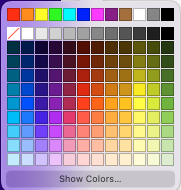
\includegraphics{png/safari_color_picker.png}
	\caption{苹果浏览器 Safari 的 HTML 调色板}
	\label{fig:1.4.2}
\end{figure}

SVG\index{SVG, Scalable Vector Graphics} 1.1中定义了148 种颜色的英文名\footnote{ \texttt{https://www.w3.org/TR/SVG11/types.html}}, 
后来也包括在了 CSS \footnote{Cascade Style Sheet: 在 HTML 中用来添加样式的语言.} 4 中 \footnote{ \texttt{https://www.w3.org/TR/css-color-4/}}.
所有互联网浏览器都支持 HTML/CSS 使用其中 141 种颜色的英文名.
用 Python 编程 SVG 生成的这些颜色如 图\ref{fig:1.4.3}.
但对比实际生成的颜色发现,个别用英文名生成的颜色有偏差,如 FireBrick (耐火红砖)和
VioletRed (紫红). 另外也应注意Green (绿色 \#{}008000)和Lime (鲜绿色 \#{}00FF00)的确切 RGB 定义. RGB 是我们接着要讨论的.

\begin{figure}[h]
	\centering
	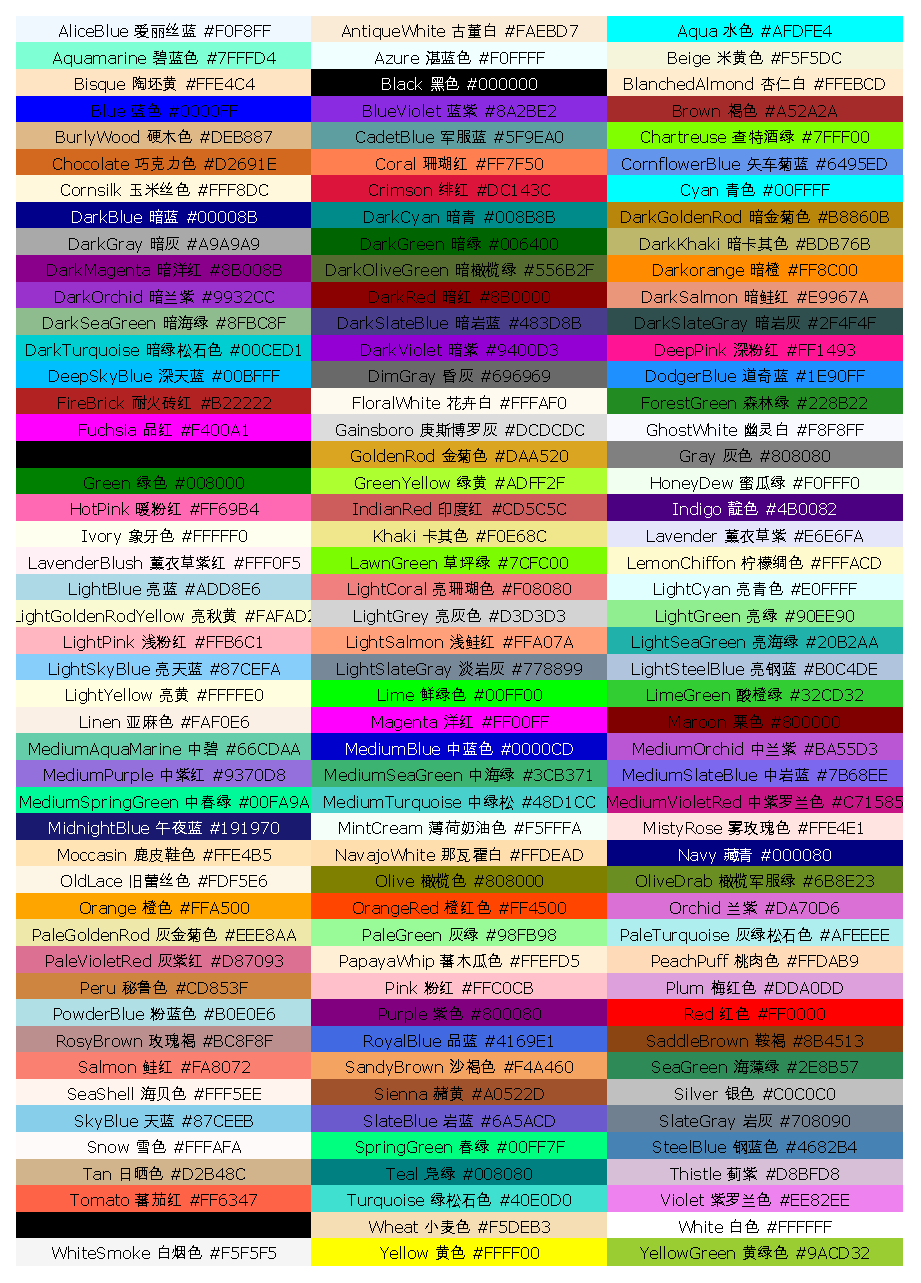
\includegraphics[width=.98\columnwidth]{eps/html_colors.eps}
	\caption{HTML/SVG 支持的 141 种颜色}
	\label{fig:1.4.3}
\end{figure}

最常用的则是 HTML
 \index{HTML 超文本标记语言} 4.01 
 最初支持的 16 种基本颜色, 如图 \ref{fig:1.4.4}. 

\begin{figure}[h]
	\centering
	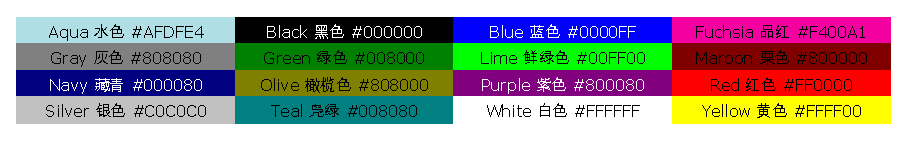
\includegraphics[width=.98\columnwidth]{eps/html_16colors.eps}
	\caption{HTML 的 16 种基本颜色}
	\label{fig:1.4.3}
\end{figure}

http://www.w3.org/TR/html5/
